\newpage
IRSTI 06.71.57
\hfill {\bfseries \href{https://doi.org/10.58805/kazutb.v.3.24-542}{https://doi.org/10.58805/kazutb.v.3.24-542}}

\sectionwithauthors{Zh.T. Konurbaeva, S.N. Suieubayeva, A.M. Zakimova, L.A. Mezentseva, A.Zh. Turegeldinova, B.B. Amralinova}{PROSPECTS FOR THE DEVELOPMENT OF ECOTOURISM IN THE EAST KAZAKHSTAN REGION IN THE CONTEXT OF IMPLEMENTING THE CONCEPT OF SUSTAINABLE DEVELOPMENT OF THE REPUBLIC OF KAZAKHSTAN}

\begin{center}
{\bfseries \textsuperscript{1}Zh.T. Konurbaeva, \textsuperscript{1}S.N.
Suieubayeva, \textsuperscript{1}A.M. Zakimova, \textsuperscript{1}L.A.
Mezentseva, \textsuperscript{2}A.Zh. Turegeldinova\envelope,
\textsuperscript{2}B.B. Amralinova}

\textsuperscript{1}D. Serikbayev East Kazakhstan Technical University,
Ust-Kamenogorsk, Kazakhstan,

\textsuperscript{2}Kazakh National Research Technical University named
after K.I. Satpayev, Almaty, Kazakhstan
\end{center}

\envelope Correspondent-author:
a.turegeldinova@satbayev.university

This study is aimed at analyzing the development of ecological tourism
in the natural territories of the East Kazakhstan Region (EKR) through a
systemic approach to the implementation of the national concept of
sustainable economic development in the Republic of Kazakhstan. The
objective of the study is to conduct a comprehensive analysis and
develop a strategy for the advancement of ecological tourism in this
region. The research is based on the interrelation and influence of
factors such as natural territories and tourist infrastructure. To
achieve this objective, various research methods were employed,
including the search for scientific materials across different platforms
and a literature review on the research topic. The search for materials
was conducted over three months, from January to May 2024. The research
also incorporated both domestic and international experiences in
sustainable tourism development. Additionally, the study involved a
comparative analysis, SWOT analysis, and correlation-regression analysis
of the impact of various tourism industry indicators on the
region\textquotesingle s GDP. The research findings emphasize the
importance of preserving the natural and cultural heritage, as well as
biodiversity, during the development of ecotourism, highlighting the
significance of sustainable resource use, adherence to environmental
standards, and principles of environmental responsibility. The study
also underscores the critical role of local tour operators and the
population in the development of ecotourism to preserve cultural
heritage and ensure the sustainable development of ecological tourism in
the East Kazakhstan Region, within the framework of the implementation
of the sustainable economic development concept of the Republic of
Kazakhstan.

{\bfseries Key words:} sustainable tourism, ecotourism, destination,
natural resources, cultural heritage, tourist infrastructure.

\sectionheading{ЭКОТУРИЗМНІҢ ДАМУ БОЛАШАҒЫ ШЫҒЫС ҚАЗАҚСТАН ОБЛЫСЫ ҚАЗАҚСТАН РЕСПУБЛИКАСЫНЫҢ ТҰРАҚТЫ ДАМУ КОНЦЕПЦИЯСЫН ЖҮЗЕГЕ АСЫРУ ЖАҒДАЙЫНДА}

\begin{center}
{\bfseries \textsuperscript{1}Ж.Т. Қоңырбаева, \textsuperscript{1}С.Н.
Сүйеубаева, \textsuperscript{1}А.М. Закимова, \textsuperscript{1}Л.А.
Мезенцева,}

{\bfseries \textsuperscript{2}А.Ж. Төрегелдинова\envelope,
\textsuperscript{2}Б.Б. Амралинова}

\textsuperscript{1}Д. Серікбаев атындағы Шығыс Қазақстан техникалық
университеті, Өскемен, Қазақстан,

\textsuperscript{2}Қ.И. атындағы Қазақ ұлттық зерттеу техникалық
университеті. Сәтбаев, Алматы, Қазақстан,

e-mail: a.turegeldinova@satbayev.university
\end{center}

Зерттеу Шығыс Қазақстан облысының (ШҚО) табиғи аумақтарында экологиялық
туризмнің дамуын талдауға бағытталған, бұл Қазақстан Республикасының
ұлттық тұрақты экономикалық даму тұжырымдамасын жүзеге асыру үшін
жүйелік тәсілді қолдануды көздейді. Зерттеудің мақсаты -- осы аймақта
экологиялық туризмнің дамуына кешенді талдау жасау және стратегия
әзірлеу. Зерттеу табиғи аумақтар мен туристік инфрақұрылым факторларының
өзара байланысы мен әсеріне негізделген. Мақсатқа жету үшін әртүрлі
зерттеу әдістері қолданылды: ғылыми материалдарды әртүрлі
платформалардан іздеу жүргізіліп, зерттеу тақырыбы бойынша әдеби шолу
жасалды. Материалдарды іздеу үш ай бойы жүргізілді: 2024 жылдың
қаңтарынан мамырына дейін. Тұрақты туризмнің дамуына арналған
материалдарда отандық және шетелдік тәжірибе зерттелді. Сонымен қатар,
зерттеу барысында Шығыс Қазақстан облысындағы экологиялық туризмнің
дамуына салыстырмалы талдау және SWOT-талдау жүргізілді, сондай-ақ,
туристік саланың әртүрлі көрсеткіш-факторларының өңірдің ЖІӨ-не әсер
етуіне корреляциялық-регрессиялық талдау жасалды. Зерттеу нәтижелері
экотуризмді дамыту барысында табиғи-мәдени ұлттық мұраны және
биологиялық әртүрлілікті сақтауға негізделген, бұл ресурстарды тұрақты
пайдаланудың маңыздылығын, экологиялық стандарттарды сақтау және
экологиялық жауапкершілік қағидаттарын баса көрсетеді. Сондай-ақ,
экологиялық туризмді дамытуға жергілікті туроператорлар мен халықтың
қатысуы мәдени мұраны сақтауда және Шығыс Қазақстан облысында
экологиялық туризмді тұрақты дамытуда маңызды рөл атқаратыны атап
өтіледі.

{\bfseries Түйін сөздер:} тұрақты туризм, экотуризм, дестинация, табиғи
ресурстар, мәдени мұра, туристік инфрақұрылым.

\sectionheading{ПЕРСПЕКТИВЫ РАЗВИТИЯ ЭКОТУРИЗМА ВОСТОЧНО-КАЗАХСТАНСКОЙ ОБЛАСТИ В УСЛОВИЯХ РЕАЛИЗАЦИИ КОНЦЕПЦИИ УСТОЙЧИВОГО РАЗВИТИЯ РЕСПУБЛИКИ КАЗАХСТАН}

\begin{center}
{\bfseries \textsuperscript{1}Ж.Т.Конурбаева,
\textsuperscript{1}С.Н.Суйеубаева, \textsuperscript{1}А.М.Закимова,
\textsuperscript{1}Л.А.Мезенцева,\\
\textsuperscript{2}А.Ж.Турегельдинова\envelope,
\textsuperscript{2}Б.Б. Амралинова}

\textsuperscript{1}Восточно-Казахстанский технический университет им.
Д.Серикбаева, Усть-Каменогорск, Казахстан,

\textsuperscript{2}Казахский национальный исследовательский технический
университет им. К.И.Сатпаева,\\
Алматы, Казахстан

e-mail: a.turegeldinova@satbayev.university
\end{center}

Исследование направлено на анализ развития экологического туризма на
природных территориях Восточно-Казахстанской области (ВКО) с
использованием системного подхода для реализации национальной концепции
устойчивого развития экономики Республики Казахстан. Цель исследования
заключается в комплексном анализе и разработке стратегии развития
экологического туризма в данном регионе. Исследование основывается на
взаимосвязи и влиянии факторов: природных территорий и туристской
инфраструктуры. Для достижения цели были применены различные методы
исследования: проведён поиск научных материалов на различных платформах
и сделан литературный обзор по теме исследования. Поиск материалов
проводился в течение трёх месяцев: с января по май 2024 г. На
материалах, посвященных теме развития устойчивого туризма, был изучен
отечественный и зарубежный опыт. Также в ходе исследования был проведён
сравнительный анализ и SWOT-анализ развития экологического туризма на
территории Восточно-Казахстанской области, а также выполнен
корреляционно-регрессионный анализ влияния на ВВП региона различных
показателей-факторов из сферы туристской отрасли. Результаты
исследования основываются на сохранении природно-культурного
национального наследия и биологического разнообразия при развитии
экотуризма, которые подчеркивают важность устойчивого использования
ресурсов, соблюдения экологических стандартов и принципов экологической
ответственности. Также отмечается важная роль участия местных
туроператоров и населения в развитии экотуризма для сохранения
культурного наследия, обеспечения устойчивого развития экологического
туризма в Восточно-Казахстанской области в рамках реализации концепции
устойчивого развития экономики Республики Казахстан.

{\bfseries Ключевые слова:} устойчивый туризм, экотуризм, дестинация,
природные ресурсы, культурное наследие, туристская инфраструктура.

\begin{multicols}{2}
{\bfseries Introduction} Tourism is one of the fastest-growing and most
significant industries globally, serving as a primary source of income
for many countries. Sustainable tourism is grounded in the principle of
caring for the environment, society, and the economy. According to a
report on environmentally safe travel published by Booking.com in honor
of Earth Day 2023, 87\% of travelers worldwide expressed a desire to
travel sustainably. Sustainable tourism encompasses practices aimed at
minimizing negative impacts while maximizing positive outcomes. It
considers the needs of tourists as well as the requirements of host
communities, local businesses, and the environment, thereby contributing
to sustainable methods of transportation, accommodation in more
environmentally friendly hotels, and the consumption of local and
eco-friendly food products.

The positive impact on the destination (areas prioritized for
development) includes job creation, the preservation and interpretation
of cultural heritage, protection of pristine nature, and restoration of
natural landscapes, among others. Conversely, negative consequences may
include economic leakage and environmental degradation {[}1{]}.

Sustainable tourism is defined by the United Nations Environment Program
and the World Tourism Organization as "tourism that fully considers its
current and future economic, social, and environmental impacts,
addressing the needs of visitors, the industry, the environment, and
host communities" {[}2{]}. Furthermore, sustainable tourism "refers to
the environmental, economic, and socio-cultural aspects of tourism
development, and it is necessary to establish an appropriate balance
between these three aspects to ensure its long-term sustainability."

The World Tourism Organization also defines sustainable tourism as
"sustainable development that meets the needs of current tourists and
host regions while protecting and enhancing opportunities for the
future" {[}2{]}. It is expected that this will lead to the management of
all resources in such a way that economic, social, and aesthetic needs
can be met while preserving cultural integrity, essential ecological
processes, biological diversity, and life-support systems.

The growth of the global population, coupled with the irrational use of
natural resources, exerts a destructive impact on our planet, leading to
climate change, destruction of nature, and increased pollution levels.
Therefore, one of the sustainable development goals is to transform
current unsustainable production and consumption patterns into those
that do not harm the environment and resources.

Challenges and Prospects in Kazakhstan's Tourism Sector The Kazakhstan
Tourism Association (KTA) believes that the challenges faced by the
tourism industry can only be resolved through strong governmental
support:

\begin{itemize}
\item
  the tourism infrastructure requires updating and refinement, including
  roads, airports, and hotels;
\item
  Kazakhstan lacks small aviation services for tourists and helicopter
  tours;
\item
  the tourist transportation system, especially in mountainous areas, is
  outdated, and modern, reliable, and comfortable buses are needed;
\item
  a more active marketing campaign is necessary to attract foreign
  tourists, as well as support for tourists from countries not included
  in the visa-free list;
\item
  efforts to develop tourism need to be intensified in the regions,
  including in the East Kazakhstan Region.
\end{itemize}

Another significant issue is the lack of qualified personnel in the
industry. According to the Institute of Economic Research (ERI), by the
end of the 2022-2023 academic year, the number of students enrolled in
educational programs such as "Tourism," "Cultural and Leisure
Activities," and "Restaurant and Hotel Management" in Kazakhstan
amounted to only 31 individuals. At the same time, the number of
graduates in these specialties was only 1,760, which constitutes 11\% of
the total number of bachelor\textquotesingle s degree graduates across
all programs.

In July 2023, the Concept for the Development of the Tourism Industry
for 2023-2029 was adopted in Kazakhstan. It aims to increase employment
in this sector to 800,000 people and grow the gross value added in the
industry to 6 trillion tenge. It is also planned to increase investment
growth in accommodation and catering services to 260 billion tenge. All
these measures are expected to increase the number of domestic tourists
to 11 million by 2030 and inbound tourists to 4 million {[}3{]}.

Systemic Approach to Ecotourism Development An essential aspect of a
systematic approach to studying the problems of ecotourism development
is considering the seasonality of tourist demand and its distribution in
the East Kazakhstan region, allowing for more efficient use of available
resources and preventing excessive pressure on the
region\textquotesingle s ecosystems. The introduction of systematic
analysis in the development of ecological tourism in the natural
territories of the East Kazakhstan region will contribute to the
sustainable development of the region\textquotesingle s economy and the
preservation of its unique natural and historical heritage.

The East Kazakhstan region has significant potential for developing
various types of tourism, ranging from ecological to business tourism.
This is facilitated by the rich history of the region, which has left
many archaeological and historical monuments on its territory. This is
ensured by the unique geographical location, where untouched corners of
nature can be found in various landscapes, including on the Kalbinsky
trail, where adventure tourism can be developed and implemented. This
type of tourism is ideal for mountain explorers, adventure enthusiasts,
and fans of an active lifestyle. It includes activities such as hiking,
trekking, canyoning, exploring caves, diving, jeep tours, buggy tours,
and more, all directly related to discovering new things and overcoming
challenges.

Historical and Cultural Significance The territory of East Kazakhstan is
the cradle of Turkic civilization. The region is home to more than 300
historical monuments. One unique archaeological site, unparalleled in
Kazakhstan, is the Berel Mounds (Valley of the Kings) located in the
Katon-Karagay district.

It is necessary to enhance the investment appeal of the region by
developing a tourism cluster, which will allow for profit generation,
increase tax revenues, and create new jobs in the region.

{\bfseries Materials and Methods} The source materials include the results
of a marketing study conducted in the winter of 2024, where the
respondents were residents of three countries: Kazakhstan, Russia, and
China. The survey was conducted anonymously using the Google Forms
platform. The technological cycle included six components: defining the
research goal, developing the questionnaire, piloting, making
adjustments, launching and conducting the survey, and evaluating and
interpreting the results. The preferences of consumers who had
undertaken tourist trips and received hospitality services were
identified during the marketing study. The research methods included
surveys, data grouping, comparison, and ranking.

The purpose of this research is to identify, analyze, and classify
various factors influencing the development of ecotourism in the EKR and
to analyze these factors based on a comprehensive analysis and the
development of a strategy for ecological tourism development in the
natural territories of the East Kazakhstan Region. The main focus is on
applying a systematic approach that allows for the consideration of
natural territories and tourist infrastructure in their interrelation,
taking into account all factors and influences.

The research methodology included a questionnaire survey of Kazakh and
foreign experts in the field of tourism services. Structural-functional
analysis, cluster analysis, object-oriented approach,
economic-statistical methods of data collection and processing,
traditional methods of comparison and generalization, and
correlation-regression analysis of the influence of factor indicators on
the final resulting indicator were used.

Additionally, structural-content analysis of texts describing the
natural landscapes of Kazakhstan and the EKR, in particular, expert
assessments, self-report methods, and extrapolation system methods were
employed.

The research involved a scientific-methodological analysis, including
thematic studies and a literature review. The significance of the
presented indicators was studied based on the results of the
questionnaire survey. Conclusions and recommendations for the
development of tourism in the East Kazakhstan Region and general
recommendations for further development of ecotourism in the Kalbinsky
Ridge area are offered.

In addition to the comparative analysis, a SWOT analysis was also
conducted during the research. These methods provided additional
information and allowed for comparing the advantages and disadvantages
of various approaches and practices.

The chosen research topic is highly relevant in the current conditions
of sustainable tourism development, due to the growing interest in
ecological domestic tourism.

The methodological and theoretical basis of the research is the
system-structural analysis as an expression of dialectics.
Structural-content analysis of various interpretations of the concept of
"sustainable tourism" showed that it is advisable to include in the list
of defining characteristics of sustainable ecotourism the following
features:

\begin{enumerate}
\def\labelenumi{\arabic{enumi})}
\item
  Ensure the optimal use of natural resources, which are the main
  element of tourism development;
\item
  Respect and preserve cultural heritage and traditional values,
  contribute to intercultural understanding and tolerance;
\item
  Provide and fairly distribute socio-economic benefits for all
  participants: employment, income opportunities, social security.
\end{enumerate}

{\bfseries Results and Discussion} The literature review analyzed several
studies dedicated to various aspects of tourism development in
Kazakhstan and the East Kazakhstan Region in particular. The authors of
the studies consider various factors influencing the development of
domestic ecotourism and offer recommendations and strategies for
sustainable development to enhance the efficiency of the tourism
industry in the region {[}4-6{]}.

Global tourism is rapidly recovering after the pandemic {[}7{]}.
According to the Bureau of National Statistics, the number of tourists
in Kazakhstan in 2023 exceeded 62 million people. On September 1, 2023,
in his Address, the President of Kazakhstan, Kassym-Jomart Tokayev,
noted that "breakthrough projects should be implemented in the tourism
sector." Indeed, in the latest global tourism ranking (The World
Economic Forum), Kazakhstan currently ranks 66th out of 117 countries
worldwide (previously, Kazakhstan held the 80th position) {[}8{]}. The
state needs to invest in the development of local tourism, which will
lead to a revival in the travel industry.

Rashida Shaikenova, Director of the Kazakhstan Tourism Association
(KTA), believes that foreigners have started coming to Kazakhstan not
only in summer but also throughout the year. Additionally, domestic
tourism has become more active, which business has immediately responded
to: local investors have begun investing in the tourism sector {[}9{]}.
The second positive development is that tourism worldwide is finally
returning to pre-pandemic levels. According to forecasts, in 2024,
tourists are expected to make 15 billion trips globally -- more than in
2019. This favorable trend is already reflected in Kazakhstan. The third
important factor is the declared Year of Chinese Tourism in Kazakhstan.
The Ministry of Tourism and Sports of the Republic of Kazakhstan has
developed a comprehensive plan that includes about 35 events covering
major cities in China: Beijing, Xi\textquotesingle an, Shanghai, Urumqi,
Hong Kong, Hangzhou, Chengdu. Tourists from China have already entered
the TOP-5 tourists who visited Kazakhstan in 2023: according to
statistics for the first nine months of 2023, the total number of
visitors from China to Kazakhstan exceeded 200,000 people {[}9{]}.

For the first half of 2023, the amount of taxes from tourism amounted to
208 billion tenge. In 2023, tourism taxes amounted to 389 billion tenge.
This indicates that tourism has become a significant source of income.
According to the World Travel \& Tourism Council (WTTC), the share of
tourism in Kazakhstan\textquotesingle s GDP in 2022 reached 3.9\% of
GDP, and the country aims to increase the share of tourism in GDP to 8\%
by 2025 {[}10{]}.

Over the past few years, the list of tourist destinations in Kazakhstan
has doubled in table 1.
\end{multicols}

\begin{table}[H]
\caption*{Table 1 -- Ranking of priority tourism development areas in Kazakhstan by region}
\centering
\begin{tabular}{|l|l|l|}
\hline
№  & Tourist areas                       & Name of the settlement   \\ \hline
1  & Khan Ordasy                         & West Kazakhstan region   \\ \hline
2  & Kargalinskoye reservoir             & Aktobe region            \\ \hline
3  & Shchuchinsko-Borovskaya resort area & Akmola region            \\ \hline
4  & Akbura                              & Akmola region            \\ \hline
5  & Imantau-Shalkar resort area         & North Kazakhstan region  \\ \hline
6  & Bayanaul                            & Pavlodar region          \\ \hline
7  & Katon-Karagay resort area           & East Kazakhstan region   \\ \hline
8  & Alakol resort area                  & Abai and Zhetisu regions \\ \hline
9  & Turgen                              & Almaty and Almaty region \\ \hline
10 & Kaskelen ski complex                & Almaty and Almaty region \\ \hline
11 & Koksai Resort                       & Zhambyl region           \\ \hline
12 & Lake Balkhash                       & Karaganda region         \\ \hline
13 & Turkestan                           & Turkestan region         \\ \hline
14 & Baikonur Cosmodrome                 & Kyzylorda region         \\ \hline
15 & Ulytau village                      & Ulytau region            \\ \hline
16 & Warm Beach                          & Mangistau region         \\ \hline
17 & Sarayshik settlement                & Atyrau region            \\ \hline
18 & Center for Gastronomic Tourism      & Shymkent                 \\ \hline
19 & Expo Tourist Area                   & Astana                   \\ \hline
\end{tabular}
\end{table}

It should be noted that at present, thirteen new global trends in
tourism development have emerged shown in table 2.

\begin{longtable}[c]{|l|p{0.2\textwidth}|p{0.7\textwidth}|}
\caption*{Table 2 -- Characteristics of new tourism trends} \\
\hline
№ &
  Trend name &
  Characteristics of the trend \\ \hline
\endfirsthead
%
\endhead
%
1 &
  Sustainable tourism and conscious travel &
  Travel that minimizes impact on nature; supports regional economies and local residents. For hotels, sustainability includes using local products in the restaurant, implementing eco-friendly practices, saving energy, and sorting waste; hosting events that introduce local traditions, crafts, etc. \\ \hline
2 &
  Immersion in local culture &
  Involving tourists in the life of the local population rather than observing it; growing interest in culture and history. A way to follow this trend is to connect with local communities. \\ \hline
3 &
  Seeking unique gastronomic experiences &
  Gaining unique culinary experiences: the beauty of presentation, aroma, and taste of food, the atmosphere of the place. Gastronomic themes add color to the promotional campaigns of regions. \\ \hline
4 &
  Self-discovery and learning new skills &
  Acquiring new knowledge and skills, developing wellness programs aimed at helping participants achieve harmony, develop creativity and communication skills, enrich their inner world. \\ \hline
5 &
  Flexible booking and payment conditions &
  The COVID-19 pandemic has heightened the uncertainty factor in travel planning. It is necessary to offer booking conditions that allow tourists to change the date and/or destination without significant penalties. \\ \hline
6 &
  Places where famous movies or TV series were filmed &
  Locations where "star" films were shot - tourist attractions. In Kazakhstan, this is the village of Teriberka. Interactive quests and reconstructions of scenes from films will add uniqueness to tours. \\ \hline
7 &
  Travel for special occasions &
  Significant personal events become reasons for travel. \\ \hline
8 &
  Emotional balance restoration &
  Growing demand for digital detox programs using practices for physical and mental recovery. \\ \hline
9 &
  Spontaneous travel &
  Related to tourists' desire to explore unknown places and enjoy unplanned trips; the appeal of last-minute tours. \\ \hline
10 &
  Countries and regions with a temperate climate &
  This trend arose in response to climate changes, due to which traditional beach resorts sometimes become too hot for comfortable rest; fans of cooler climates visit mountain resorts. \\ \hline
11 &
  Visiting unexplored countries and regions (instead of popular ones) &
  Choosing alternative destinations instead of familiar ones (this trend applies to both beach resorts and mountains). \\ \hline
12 &
  Attributes of "beautiful life" for budget travelers &
  A way to relax comfortably and brightly without significant expenses. The trend requires a balanced approach from tour operators and hotels in forming offers: base prices for trips accessible to a wide range of consumers should be complemented by a wide list of high-quality services. \\ \hline
13 &
  Use of innovative technologies in travel planning &
  Statistics from Booking – 48\% of travelers trust artificial intelligence (AI) to plan their trips (from 8\% in the UK to 63\% in the US). AI can quickly analyze large volumes of information, provide personalized recommendations, and optimize routes. \\ \hline
\caption*{\normalfont \emph{Sources: Expedia Group,~Skyscanner,~Booking}} \\
\end{longtable}

\begin{multicols}{2}
Tourism Operators and Sustainable Development Tour operators contribute
to the sustainable development of tourist areas by creating jobs for
local residents. Additionally, they can include visits to special
attractions (museums, workshops, etc.) that support local communities in
their programs, and give tourists the opportunity to engage in
environmental projects. All this will allow guests to feel involved in
preserving the cultural and natural heritage of the regions they visit.
Promoting programs based on the principles of sustainable tourism can
become a unique feature that distinguishes the tour
operator\textquotesingle s product {[}11{]}.

Competent marketing is crucial for the success of creating a new trend:
in an advertising campaign, it is important to show the advantages of a
new destination, emphasizing its uniqueness and, at the same time, its
similarity to what is already known to the market {[}12{]}.

The results of the literature review on the research topic can be used
to form strategies and policies for the development of ecological
tourism in the East Kazakhstan Region of the Republic of Kazakhstan. As
EKR borders Russia and China, this gives good prerequisites for foreign
travelers to visit the region. There are also excellent prospects for
the domestic tourist product of EKR. Among the main tasks that will
bring success to travel agencies in this area are the development of
roadside services, the opening of new accommodation facilities, and the
improvement of existing ones. In the first place, these are private
mini-hotels and guest houses. Tourism statistics in Kazakhstan claim
that they have almost equaled traditional hotels in popularity.

From September 21 to 26, 2023, filming of the educational travel program
"Orel and Reshka. Kazakhs" took place in the Katon-Karagay district. The
filming was organized through the joint work with local executive bodies
in such tourist destinations as: Osinovsky Pass, Rakhmanovskie Keys, the
old Austrian road, and others. The episode is scheduled to air in the
second quarter of 2024 on the "Jibek Joly" TV channel.

Several ski resorts are located near the cities of Ust-Kamenogorsk and
Ridder: "Nurtau" and "Altai Alps" are the most famous among them.

"In East Kazakhstan, we have three major destinations for the
development of ecotourism -- Katon-Karagay, Ridder, and the Ulan
district. Plus, the fourth -- Ust-Kamenogorsk as the logistics hub of
tourism in EKR," noted Mukhtar Toibazarov. The entrepreneur said that
currently, about 15 antler therapy centers operate in EKR, which can
receive no more than 6,750 people per season. All guest houses and
hotels in the Katon-Karagay district can accommodate no more than 3,000
people.

"The entire population of Ulken Naryn is about 23,000 people. And for
tourism to benefit the population of border areas, for it to be
significant, we need tourists. And if there were at least 25,000
tourists, the entire district would feel it. If we had at least
70,000-100,000 tourists throughout EKR, the whole region would feel it,
all hotels in Ust-Kamenogorsk would be filled, all restaurants would be
full, and there would be a need to build new ones," concluded Mukhtar
Toibazarov.

From January to September 2023, Kazakhstan was visited by 37\% more
foreign tourists than during the same period in 2022 - 8,349 thousand
people - according to the Ministry of Tourism and Sports of the Republic
of Kazakhstan. According to its data, most tourists in the first nine
months of 2023 came to Kazakhstan from {[}13{]}:

\begin{itemize}
\item
  Russia (356,850, 12\% more than in January-September 2022);
\item
  China (75,131, twice as many);
\item
  Turkey (41,134, 2\% less);
\item
  India (34,757, 34 times more);
\item
  USA (28,160, 15 times more).
\end{itemize}

The structure of visitors to the Republic of Kazakhstan is presented in
Figure 1.

\begin{figure}[H]
	\centering
	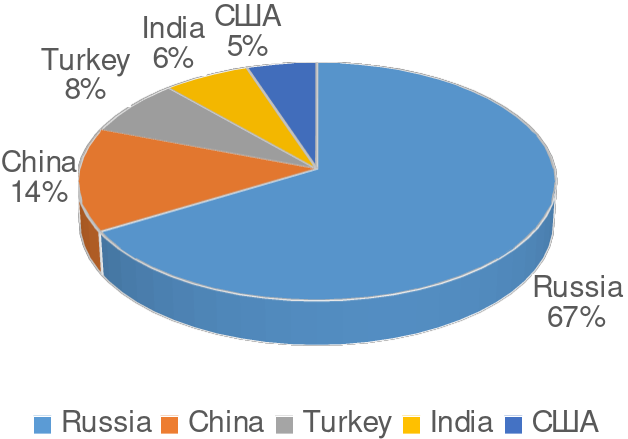
\includegraphics[width=0.4\textwidth]{assets/340.2}
	\caption*{Figure 1 - Structure of Visitors to the Republic of Kazakhstan in 2023}
\end{figure}

In Kazakhstan, the tourist tax for foreigners was canceled. By order of
the Minister of Tourism and Sports of the Republic of Kazakhstan dated
December 27, 2023, No. 347, changes were made to the rules for paying
the tourist tax for foreigners, according to which a zero rate will be
applied throughout Kazakhstan. The tourist tax bedtax was introduced in
Kazakhstan at the beginning of 2023. The main goal of its introduction
was to accumulate funds for the development of regional tourism in
Kazakhstan. The minimum bedtax rate was 0.3 MCI (1,035 tenge in 2023),
the maximum - 0.5 MCI (1,725 tenge) depending on the growth of tourists
{[}10{]}.

In 2024, Kazakhstan will spend 586 million tenge to attract foreign
tourists and promote the country\textquotesingle s tourist image
(according to the press service of the Ministry of Tourism and Sports of
the Republic of Kazakhstan) {[}14{]}. At a government meeting, Minister
Ermek Marzhikpaev emphasized that after the pandemic, the tourism sector
worldwide is actively competing for tourists\textquotesingle{}
attention. States are investing significant funds in advertising and
promoting their countries. Emphasis will be placed on the Kazakhstan
Tourism Year in China, increasing the number of international
exhibitions, attracting foreign media. A mechanism is also being
developed for off-budget financing of large-scale events in the tourism
sector through the Corporate Fund for Supporting the Tourism and Sports
Industry.

Kazakhstan ranked 5th on the list of the best countries for adventure
tourism according to the British Backpacker Society. This is fully
justified by the vast variety of suitable natural spaces and its great
potential. EKR has 24 tourism sites, but it is necessary to develop the
25th - the Kalbinsky Ridge {[}14{]}.

An excellent idea for the development of sustainable tourism in EKR
would be the cooperation of recreation bases - a kind of "exchange of
tourists" and the development of new interesting tourist routes. We
offer several real initiatives that can change the situation in the
tourism industry. Among them:

\begin{itemize}
\item
  Road repairs (2024, the head of EKR declared the Year of Roads) to
  major tourist sites;
\item
  Installation of sanitary and hygiene units every 50 km of roads, with
  subsequent maintenance;
\item
  Construction of observation platforms in beautiful locations in the
  region;
\item
  Opening airports in Katon-Karagay and Ulken Naryn;
\item
  Opening more guest houses and yurts in villages;
\item
  Training local residents in service rules and techniques, preparing
  guides and tour guides in special profile courses;
\item
  Opening a craftsman center for the production of yurts from local
  materials;
\item
  Laying safe trails for hiking, horse, and cycling routes (e.g., along
  the Kalbinsky Ridge);
\item
  Opening a modern visitor center in Ust-Kamenogorsk with
  representatives of tour operator companies;
\item
  Holding international image events and festivals in EKR (climbing
  Kyzyl-Tas, berkutchi festival, "Taste of Altai" cuisine festival);
\item
  Creating three winter clusters for active winter recreation and skiing
  in Ridder, the Ivanovsky Ridge, Gornaya Ulbinka, and near the regional
  center;
\item
  Improving logistics for the uninterrupted delivery of tourists from
  Ust-Kamenogorsk to vacation spots.
\end{itemize}
\end{multicols}

\begin{table}[H]
\caption*{Table 3 -- Key Data on Accommodation and Visitors in EKR for 2023}
\centering
\begin{tabular}{|p{0.6\textwidth}|l|}
\hline
Single capacity (beds) of accommodation facilities, units & 33629 \\ \hline
Hotel occupancy rate (beds), \% & 27,6 \\ \hline
Visitors served by accommodation facilities for domestic tourism (residents), persons. & 582948 \\ \hline
Visitors served by accommodation facilities for domestic tourism (residents) persons, persons & 29741 \\ \hline
\end{tabular}
\end{table}

\begin{multicols}{2}
The East Kazakhstan Region is one of the promising regions for inbound
tourism. Tourism statistics in Kazakhstan indicate that travelers visit
EKR for a variety of purposes (table 3). Family vacations are usually
organized at Lake Alakol with its famous black pebble beaches and the
healing properties of its waters {[}13{]}. You can also go for health
purposes to the Katon-Karagay National Park, which houses many
sanatoriums, rest houses, and antler therapy centers. People also go
there to admire natural beauty and visit historical and cultural sites,
of which there are many.

Statistics show that most travelers head to the mountainous areas of the
East Kazakhstan Region. Conditions for developing this market niche are
the most favorable here. In addition to the Altai spurs, the region
includes the Sauyr-Tarbagatai Mountains, some of the most beautiful in
Central Asia, with peaks covered with eternal glaciers on their northern
side. The Kalbinsky Mountain Ridge, with its powerful strip of granite
intrusions covered with pine forests, is also popular among tourists.

One of the most important factors for attracting tourists is the level
of awareness of the region\textquotesingle s residents about the
existence of sites of interest and their specific features. In the
survey, respondents were asked to mark the places in the East Kazakhstan
Region they had heard of and the places they had visited. The survey
results are presented in Table 4.
\end{multicols}

\begin{table}[H]
\caption*{Table 4 - Assessment of the Awareness of 10 Recreation Sites in the East Kazakhstan Region}
\centering
\begin{tabular}{|l|ll|}
\hline
\multirow{2}{*}{What places have you heard about / What places have you been to} & \multicolumn{2}{l|}{Share of respondents, \%} \\ \cline{2-3} 
 & \multicolumn{1}{l|}{Heard} & Visited \\ \hline
Sanatorium "Rakhmanovskie Klyuchi" & \multicolumn{1}{l|}{17,3} & 3,9 \\ \hline
"Sibinsky Lakes" & \multicolumn{1}{l|}{19,1} & 8,1 \\ \hline
Bukhtarma Reservoir Heard & \multicolumn{1}{l|}{40,3} & 13,2 \\ \hline
Ski complexes "Altai Alps" and "Nurtau" & \multicolumn{1}{l|}{20,6} & 11,1 \\ \hline
Lake Alakol & \multicolumn{1}{l|}{39,1} & 15,6 \\ \hline
"Valley of the Kings" Katon-Karagay National Park & \multicolumn{1}{l|}{11,5} & 5,4 \\ \hline
Lake Zaisan & \multicolumn{1}{l|}{12,7} & 6 \\ \hline
Lake Markakol & \multicolumn{1}{l|}{7,9} & 3,9 \\ \hline
Kalbinsky Ridge & \multicolumn{1}{l|}{5,8} & 3,9 \\ \hline
Kiin-Kerish Gorge & \multicolumn{1}{l|}{5,8} & 2,1 \\ \hline
No awareness / Never visited & \multicolumn{1}{l|}{30} & 63,7 \\ \hline
\end{tabular}
\end{table}

\begin{multicols}{2}
As can be seen from the survey results, the most well-known sites among
residents of Kazakhstan, Russia, and China are "Bukhtarma Reservoir"
(40.3\%), Lake Alakol (39.1\%), and the ski complexes "Altai Alps" and
"Nurtau" (20.6\%). At the same time, 30\% of respondents from
territories bordering East Kazakhstan had never heard of any recreation
sites in East Kazakhstan. The sanatoriums "Rakhmanovskie Klyuchi"
(17.3\%) and "Sibinsky Lakes" (19.1\%) are little known to residents,
and they are practically unfamiliar with the attractions of Lake
Markakol (7.9\%), Kalbinsky Ridge, and Kiin-Kerish Gorge (both 5.8\%).

The survey shows that 15.6\% of respondents visited Lake Alakol. The
Bukhtarma Reservoir was visited by 13.2\% of respondents. The ski
complexes of EKR were visited by 11.1\% of respondents. A total of
63.7\% of respondents had never visited the recreation sites of East
Kazakhstan {[}13{]}.

The survey results indicate a lack of awareness among residents of the
three countries about the attractions of the Altai region and the need
to develop a comprehensive program for promoting ecotourism in the
region of the Altai Mountains and the Blue Lakes - the jewel of
Kazakhstan.

During the study, the authors conducted an assessment of the strengths
and weaknesses of tourism development in the East Kazakhstan Region. The
generalized results of the analysis of the dynamics and trends of
tourism services development, as well as the prerequisites for forming
practical recommendations for increasing the attractiveness of the
tourism services market, are presented in the form of a SWOT analysis
matrix (Table 5).

This analysis shows that ecological tourism has development potential in
the East Kazakhstan region but requires efforts to develop
infrastructure, increase awareness of natural resources and
environmental issues, and ensure a sustainable and responsible approach
to the tourism industry as a whole.
\end{multicols}

{\footnotesize
\begin{longtable}[c]{|p{0.57\textwidth}|p{0.37\textwidth}|}
    \caption*{Table 5 -- SWOT Analysis of Forming the Attractiveness of Tourism Services in the East Kazakhstan Region} \\
    \hline
    \textbf{Strengths} & \textbf{Weaknesses} \\ 
    \hline
    \begin{tabular}[c]{p{0.55\textwidth}}
        Production of tourism services at the lowest cost in the place of consumption; \\
        Local population's interest in developing inbound and domestic tourism; \\
        Development of new tourism services; \\
        Continuous improvement of service quality; \\
        High informatization of all participants in the tourism services market, resulting from the dynamic development of information and communication systems; \\
        Rich natural resource potential and beautiful natural landscapes; \\
        Rich historical and cultural heritage of the region; \\
        Representation of national color; \\
        Availability of a conceptual basis for developing the tourism industry in the region; \\
        Development of economic and cultural ties with all regions of Kazakhstan; \\
        Rich traditions of hospitality, experience in receiving and serving visitors; \\
        Favorable conditions for developing various types of tourism; \\
        Scientific and educational potential for training specialists in the region; \\
        Relatively stable socio-economic situation; \\
        Advertising promotion - social networks Instagram, 2GIS.
    \end{tabular}
    &
    \begin{tabular}[c]{p{0.35\textwidth}}
        Uneven distribution of natural potential, climatic conditions determine the seasonality of tourism services (summer and winter periods); \\
        High cost of the tourism product; \\
        Individualization of service provision, increasing quality requirements as a consequence of growing competition; \\
        Lack of incentives for developing inbound and domestic tourism; \\
        Lack of qualified specialists in the tourism industry; \\
        Lack of marketing activities; \\
        Unfavorable environmental situation in EKR; \\
        Weak logistical and transport infrastructure in EKR.
    \end{tabular}
    \\ \hline
    \textbf{Opportunities} & \textbf{Threats} \\ 
    \hline
    \begin{tabular}[c]{p{0.55\textwidth}}
        Continuously growing demand in this market and the emergence of new customers; \\
        Growth of economic potential through the development of new tourism services; \\
        Possibility of diversifying the tourism product; \\
        New developments and opportunities for modern types of tourism development; \\
        Possibility of developing tourism infrastructure by attracting investments; \\
        Improving service quality in all sectors of the economy; \\
        The flourishing of the services market era on a global scale; \\
        Possibility of rapid development with the restoration of pre-pandemic demand levels in the tourism services market as a whole; \\
        Sustainable domestic demand for visiting historical and cultural heritage sites; \\
        Increasing productivity of companies included in the tourism cluster, i.e., increasing innovative potential and creating new business projects; \\
        Developing new tourism products for visiting little-explored areas, such as the Kalbinsky Ridge; \\
        Expanding the range of services offered, improving service quality and tourist safety; \\
        The pandemic has led to an increase in the number of tourists engaging in active sports - mountain tourism, trekking, hiking, and walking.
    \end{tabular}
    &
    \begin{tabular}[c]{p{0.35\textwidth}}
        The emergence of new services in the market; \\
        Increasing market requirements for service quality; \\
        Changing nature of demand for various types of services; \\
        Decline in business activity due to the worsening economic situation in the country and the world; \\
        Intensifying competition in the struggle for investment resources; \\
        Availability of alternative uses for territories suitable for tourism development; \\
        Unstable demand in the tourism services market due to seasonality and other factors; \\
        Imperfection of legislation on tourism activities regulation; \\
        Difficulty attracting qualified specialists and personnel to the tourism sector; \\
        Destruction of historical and cultural monuments due to insufficient measures for their preservation; \\
        Low quality and uniformity of tourism products; \\
        Competition with other tourist destinations and regions.
    \end{tabular}
    \\ \hline
\end{longtable}
}

\begin{multicols}{2}
From January to September 2023, the East Kazakhstan Region saw the
following dynamics of key tourism indicators:

\begin{itemize}
\item
  The volume of services provided by accommodation facilities amounted
  to 47.119 million tenge (an increase of 23.5\% compared to the same
  period in 2022);
\item
  2.812 thousand citizens of Kazakhstan used accommodation services (an
  increase of 13.7\% compared to the same period in 2022);
\item
  The number of foreign tourists amounted to 147 thousand people (an
  increase of 16.6\% compared to the same period in 2022);
\item
  Investments in fixed assets in the tourism sector amounted to 9.457
  million tenge (an increase of 33.0\% compared to the same period in
  2022).
\end{itemize}

For socio-economic phenomena, it is characteristic that along with
significant factors shaping the level of the effective indicator, many
factors influence it. This indicates that the relationships between the
phenomena being studied are correlational in nature and are analytically
expressed by the function Y\textsubscript{x} = f(x). Determining the
regression equation and the strength of the relationship between the
studied phenomena constitutes the essence of correlation-regression
analysis (CRA).

The research aims to determine the dependence of tourism development on
the level of socio-economic development of the region based on
correlation-regression analysis. To build a model for forecasting the
main socio-economic indicators, which will allow managing the
sustainable development of tourism in the East Kazakhstan Region, the
correlation-regression analysis method was used based on monthly data
for 2023 (Table 6).

As the dependent variable, we define Y - the volume of income from
services provided, million tenge. The following factor indicators were
selected as explanatory variables:

X\textsubscript{1} - the number of citizens of Kazakhstan who entered
the territory of EKR, thousand people;

X\textsubscript{2} - the number of foreign tourists, thousand people;

X\textsubscript{3} - investments in fixed assets in the tourism sector,
million tenge.
\end{multicols}

\begin{table}[H]
\caption*{Table 6 -- Initial Data of Correlation-Regression Analysis}
\centering
\begin{tabular}{|l|p{0.18\textwidth}|p{0.18\textwidth}|p{0.18\textwidth}|p{0.18\textwidth}|}
\hline
Period &
  Volume of Income from Services Provided (million tenge) &
  Number of Citizens of Kazakhstan who Entered EKR (thousand people) &
  Number of Foreign Tourists (thousand people) &
  Investments in Fixed Assets in the Tourism Sector (million tenge) \\ \hline
01.01.2023 & 517,118 & 30,089 & 1,409 & 1029,577 \\ \hline
01.02.2023 & 519,496 & 30,112 & 1,612 & 1039,985 \\ \hline
01.03.2023 & 527,219 & 31,244 & 1,513 & 1049,985 \\ \hline
01.04.2023 & 526,874 & 31,189 & 1,514 & 1051,778 \\ \hline
01.05.2023 & 519,638 & 31,502 & 1,524 & 1051,258 \\ \hline
01.06.2023 & 522,237 & 31,588 & 1,526 & 1058,983 \\ \hline
01.07.2023 & 526,528 & 32,897 & 1,784 & 1057,145 \\ \hline
01.08.2023 & 523,246 & 32,421 & 1,865 & 1058,962 \\ \hline
01.09.2023 & 529,544 & 30,158 & 1,953 & 1059,327 \\ \hline
01.10.2023 & 518,788 & 30,457 & 1,757 & 1058,322 \\ \hline
01.11.2023 & 520,159 & 30,101 & 1,142 & 1059,537 \\ \hline
01.12.2023 & 522,987 & 31,105 & 1,112 & 1060,899 \\ \hline
\end{tabular}
\end{table}

\begin{multicols}{2}
To empirically verify the conceptual model, the authors conducted
Pearson correlation analysis, as all variables are continuous in nature.
All calculations were performed using the "Data Analysis" tool in
Microsoft Excel.

As a result of the calculations, it is evident that there is a strong
relationship between the amount of income from services rendered and the
number of tourists visiting the East Kazakhstan Region, as well as the
volume of investments in the tourism sector, with the correlation
coefficient R = 0.713 or 71.3\%.

The coefficient of determination D = 0.5087 or 50.87\%, meaning that
50.87\% of the variation in Y is explained by changes in
X\textsubscript{1}, X\textsubscript{2}, and X\textsubscript{3}, while
the remaining 49.13\% is influenced by other factors.

The multiple regression equation is as follows:

Y=712.443+2.526×X\textsubscript{1}+1.222×X\textsubscript{2}+0.253×X\textsubscript{3}

where 2.526 is the regression coefficient showing how much Y will change
with a one-unit change in X\textsubscript{1} (the number of citizens of
the Republic of Kazakhstan entering the East Kazakhstan Region);

1.222 is the regression coefficient showing how much Y will change with
a one-unit change in X2 (the number of foreign tourists);

0.253 is the regression coefficient showing how much Y will change with
a one-unit change in X3 (investments in fixed assets in the tourism
sector);

712.443 is the intercept in the regression equation, interpreted as the
initial value of Y.

We will assess the statistical significance of the regression equation
and its parameters using Fisher\textquotesingle s and
Student\textquotesingle s t-tests (at a 5\% significance level) and
elasticity coefficients (5\% significance level; 3 degrees of freedom).

The theoretical t-value (Ttheor) = 2.23 is the table value of the
Student\textquotesingle s coefficient. The calculated
Student\textquotesingle s t-value (T) = 6.551 \textgreater{} 2.23.

Thus, it can be concluded that the linear correlation coefficient is
significant and reliable.

The table value of Fisher\textquotesingle s criterion: F-criterion =
3.59.

The calculated F-value = 22.761 \textgreater{} 3.59, indicating that the
constructed equation is statistically significant and can be used to
calculate forecast values of income in the tourism sector of the East
Kazakhstan Region based on changes in the number of domestic and foreign
tourists, as well as the volume of investments in tourism.

{\bfseries Conclusion} The conducted research demonstrates that the East
Kazakhstan Region has tremendous potential for the development of
ecological tourism, thanks to its rich natural resources, diverse
landscapes, and unique ecosystems, including the Kalbinsky Ridge.

As recommendations for the development of tourism in the East Kazakhstan
Region, it is essential to focus on developing a system of state
regulation and support for tourism activities. The comprehensive
implementation of planned measures will contribute to an influx of
foreign tourists to the region, strengthen the material and technical
base of tourism, expand the diversity and geography of tourist routes,
stimulate other industries, and make a significant contribution to the
structural transformation of the regional economy.

Macroeconomic and political stability in Kazakhstan, along with the
organization of world-scale events, will provide a powerful impetus for
further business cooperation in the field of ecotourism. Developing a
sound strategy that considers global practices and experiences will
allow ecotourism in East Kazakhstan to become a profitable component of
the region\textquotesingle s economy.

The conducted study on the impact of the tourism sector on the economy
of the East Kazakhstan Region using correlation-regression analysis has
revealed a positive correlation between the amount of income from
services rendered and the number of tourists accommodated, as well as
the volume of investments in the tourism industry. It was found that the
development of tourism in the East Kazakhstan Region is primarily driven
by domestic tourist flows.

The results of the conducted SWOT analysis form the basis for
determining the strategic directions for the development of domestic
tourism services and improving tourism support in the East Kazakhstan
Region.

Thus, it can be concluded that the dynamic development and
transformations, equally affecting both the demand for and the supply of
tourism services, indicate a transition to a qualitatively new stage in
the development of domestic tourism in the East Kazakhstan Region.

\emph{{\bfseries Financing:} This research was conducted as part of the
implementation of the initiative project 0124РКИ0093 ``Tourism Potential
of the Natural and Historical-Cultural Complex
\textquotesingle Kalbinsky Trails\textquotesingle.''}
\end{multicols}

\begin{center}
{\bfseries References}
\end{center}


\begin{noparindent}
1.
Zakon Respubliki Kazahstan ot 13 ijunja 2001 goda № 211 «O turistskoj
dejatel\textquotesingle nosti v Respublike Kazahstan» //
Informacionno-pravovaja sistema normativnyh pravovyh aktov Respubliki
Kazahstan.

URL:https://adilet.zan.kz/rus/docs/Z010000211 (accessed:
05.01.2024) {[}in Russian{]}

2.
Tourism in the World. United Nations World Tourism Organization. URL:
https://www.unwto.org

3.
Ob utverzhdenii Koncepcii razvitija turistskoj otrasli Respubliki
Kazahstan na 2023 -- 2029 gody. Postanovlenie
Pravitel\textquotesingle stva Respubliki Kazahstan ot 28 marta 2023
goda № 262.

URL: https://adilet.zan.kz/rus/docs/P2300000262 (accessed:
03.03.2024) {[}in Russian{]}

4.
Seken, A., Duissembayev, A., Tleubayeva, A., Konurbaeva, Z.,
Suieubayeva, S. Modern potential of rural tourism development in
Kazakhstan // Journal of Environmental Management and Tourism. --
2019. --Vol. 10(6). -P. 1211--1223. DOI: 10.14505//jemt.v10.6(38).03

5.
Mutaliyeva, L., Kurmanov, N., Akisheva, A. Analysis of tourism
potential and ecological tourism

development in Kazakhstan // E3S Web
of Conferences. EDP Sciences. -- 2020. - Vol. 159. -P. 1--7.

https://doi.org/10.1051/e3sconf/202015904031

6.
Abuev A. Turizm v Kazahstane: issledovanie otrasli, problematika i
perspektiv. -2023. URL:

https://ffin.kz/research/9-turizm-v-kazakhstane-issledovanie-otrasli-problematika-i-perspektivy
(accessed: 21.07.2024)

7.
Khalid, U., Okafor, L.E., Burzynska, K. Does the size of the tourism
sector influence the economic policy response to the COVID-19
pandemic? // Current Issues in Tourism. -2021. -Vol. 24(19). -P.
2801--2820. DOI:10.1080/13683500.2021.1874311

8.
Mirovoj rejting turizma: kakoe mesto zanjal Kazahstan // Official
Website inbusiness.kz. URL:

https://inbusiness.kz/ru/last/mirovoj-rejting-turizma-kakoe-mesto-zanyal-kazahstan
(accessed: 02.08.2024)

9.
Kak prevratit\textquotesingle{} Kazahstan v turisticheskuju Mekku?
Mnenie jeksperta. // Official Website Azattyq Rýhy. URL:
https://rus.azattyq-ruhy.kz/economics/53058-kak-prevratit-kazakhstan-v-turisticheskuiu-mekku

-mnenie-eksperta
(accessed: 02.08.2024)

10.
International Tourism Highlights // Tourism Library. URL:

https://tourlib.net/wto/WTO\_highlights\_2019.pdf?ysclid=lcp2b4u0vu212952496

11.
Kajnazarova D.A., Bajmagambetova L.K. Postkovidnoe sostojanie i
razvitie turizma Kazahstana // Vestnik universiteta «Turan». -2023.
--Vol. 2. --P. 216-233.
https://doi.org/10.46914/1562-2959-2023-1-2-216-233

12.
Chernysheva A., Jakubova T. Marketingovye issledovanija i situacionnyj
analiz v 2 ch. Chast\textquotesingle{} 1. Uchebnik i praktikum dlja
akademicheskogo bakalavriata. -- Moscow: Litres, 2020. -- 244 p. ISBN
978-5-9916-8566-5

13.
Bureau of National Statistics of the Agency for Strategic Planning and
Reforms of the Republic of Kazakhstan. URL: https://www.stat.gov.kz/

14.
Bureau of National Statistics of the Agency for Strategic Planning and
Reforms of the Republic of Kazakhstan // Statistical Digest "Tourism
Statistics of Kazakhstan 2021--2023". URL:

https://stat.gov.kz/ru/industries/business-statistics/stat-tourism/
(accessed: 05.03.2024)
\end{noparindent}

\emph{{\bfseries Information about the authors}}

\begin{noparindent}
Konurbayeva Zh. - D. Serikbayev East Kazakhstan Technical University,
Candidate of Economic Sciences, Associate professor, Ust-Kamenogorsk,
Kazakhstan, e-mail: zhkonurbayeva@edu.ektu.kz;

Suieubayeva S. -D. Serikbayev East Kazakhstan Technical University,
Candidate of Economic Sciences, Associate professor, Ust-Kamenogorsk,
Kazakhstan, e-mail: suyeubaeva@mail.ru;

Zakimova A. - D. Serikbayev East Kazakhstan Technical University,
Candidate of Economic Sciences, Ust-Kamenogorsk, Kazakhstan, e-mail:
zakimovaa@mail.ru;

Mezentseva L. - D. Serikbayev East Kazakhstan Technical University,
Ust-Kamenogorsk, Kazakhstan, e-mail: Vvdovin@list.ru;

Turegeldinova A. - Kazakh National Research Technical University named
after K.I. Satpayev, Candidate of Economic Sciences, PhD, Almaty,
Kazakhstan, a.turegeldinova@satbayev.university;

Amralinova B. - Kazakh National Research Technical University named
after K.I. Satpayev, PhD, Associate professor, Almaty, Kazakhstan,
b.amralinova@satbayev.university.
\end{noparindent}

\emph{{\bfseries Сведения об авторах}}

\begin{noparindent}
Конурбаева Ж. - Восточно-Казахстанский технический университет им. Д.
Серикбаева, к.э.н., доцент, г. Усть-Каменогорск, Казахстан, e-mail:
zhkonurbayeva@edu.ektu.kz;

Суйеубаева С. - Восточно-Казахстанский технический университет им. Д.
Серикбаева, к.э.н., доцент, г. Усть-Каменогорск, Казахстан, e-mail:
suyeubaeva@mail.ru;

Закимова А. - Восточно-Казахстанский технический университет им. Д.
Серикбаева, к.э.н., доцент, г. Усть-Каменогорск, Казахстан, e-mail:
zakimovaa@mail.ru;

Мезенцева Л. - Восточно-Казахстанский технический университет им. Д.
Серикбаева, г. Усть-Каменогорск, Казахстан, e-mail: Vvdovin@list.ru;

Турегельдинова А. - Казахский национальный исследовательский технический
университет им. К.И. Сатпаев, к.э.н., PhD, Алматы, Казахстан,
a.turegeldinova@satbayev.university;

Амралинова Б. - Казахский национальный исследовательский технический
университет имени К.И. Сатпаева, к.э.н., доцент, Алматы, Казахстан,
b.amralinova@satbayev.university.
\end{noparindent}
